\chapter{Learning Rules With Numerical and Categorical Attributes}
\label{cl:intro}

\section{Interesting Rules}

In this section we formally define what kind of rules we are interested in obtaining with the algorithm proposed in
this thesis. As briefly explained in the introduction, the objective learning with numerical attributes, focusing on searching ranges in the numerical domain that satisfy support and accuracy thresholds.

Trying to learn numerical ranges for a base-rule that already satisfies accuracy threshold is considered uninteresting, as the gain would be probably small

\section{Categorical Relation Definition}

In this section, we formally define a categorical relation as used in the \graphname. 

First of all, a candidate relation must be joined with root relation's \ord{1} argument (assuming that the numerical
attribute is in the \ord{2} argument). 

A candidate categorical relation $r(x,y)$, should be equivalent a non-injective function:

$r(x,y) \equiv f : X \rightarrow Y , \quad s.t. \, |Y|<|X| $ and $ |Y|>1 \newline $
$\nexists \, g : Y \rightarrow X , \quad s.t. \, f(g(x))=x , \quad \forall x \in X$

We can define subsets of $X_i \in X$, with which of them belonging to one category $y_i \in Y$:

$X_i \subset X \quad s.t. \, X_i = \{x \in X \,|\, f(x)=y_i ,\, y_i \in Y\} \newline $
$X = \bigcup_{i=1}^{n} X_i $ and $ X_i \cap X_j = \emptyset ,\quad \forall i,j \in [1,n] ,\, i \neq j$

We can also broaden this definition by composing functional relations to a categorical or multiple categorical
relations:

If we have:

$r_1(x,y) \equiv f_1 : X \rightarrow Y$ \newline
$r_2(y,z) \equiv f_2 : Y \rightarrow Z$ 

Where at least one of them is categorical, then $r'(x,z) \equiv f : X \rightarrow Z$, where $r'(x,z)=r_2(f_1(x),z)$ is also categorical


Numerical properties can also be turned into a categorical, by simply applying a bucketing function that maps a
numerical domain into a finite set of $k$ buckets:

$b: \mathbb{N} \rightarrow B$, where $B=\{1,2,\dots ,k \}$

So a numerical property:

$r(x,y) \equiv f : X \rightarrow \mathbb{N}$ 

combined with a bucketing function $b$, $r'(x,b(y))$ would be discretized and applicable in the \graphname.

(Then talk about non-categorical relations as categorical by considering its presence/absence)

Types are also covered by this definition. If we consider $r = rdf:type$ we see that $r$ which maps entities into
types satisfies the definition presented before.

\subsection{Absence or Presence of a Relation as Categories}

Another possibility is to define categories for presence or absence of relations. With this approach, one can also
include non-categorical relations into the \graphname and have insight about how the presence or absence of such
relation affects the distribution of root's numerical attribute.

As in this thesis we are under open world assumption and we don't consider negated literals in the hypothesis, we ignore
the absence and just include the presence of relations in the lattice.


%\subsection{Notation Used}
%
%As we will see in the next sections, in the \graphname all the relations are joined by a single variable $x$. So we will denote:
%
%$r(x,y)$ as $r$
%
%$r(x,C_i) or r(C)$ as $r_i$

\section{Preprocessing}

In this section, we will present the preprocessing steps required by our proposed algorithm. It basically consists of
first building a graph with the knowlw building a joinable relations map for each of the four join patterns, according
to relations domain and range types as well as support threshold. Afterwards, we search the available categorical
properties for each numerical relation that will be used in the \graphname. At last we build the so called \graphname,
which belongs to the preprocessing step but will be discussed in the next Section s\ref{ch:lattice}.

\subsection{Relation Preprocessing}

In this step, we focus on creating for each of the four join patterns between two relations:

\begin{itemize}
 \item Argument 1 on Argument 1: e.g. \emph{hasIncome(\textbf{x},y)hasAge(\textbf{x},z)}
 \item Argument 1 on Argument 2: e.g. \emph{hasIncome(\textbf{x},y)isMarriedTo(z,\textbf{x})}
 \item Argument 2 on Argument 1: e.g. \emph{livesIn(y,\textbf{x})isLocatedIn(\textbf{x},z)}
 \item Argument 2 on Argument 2: e.g. \emph{livesIn(y,\textbf{x})wasBornIn(z,\textbf{x})}
\end{itemize}

\subsubsection{Exploiting Relation Range and Domain Types}

A knowledge base is expected to have an ontology defining the structure of the stored data (the types of entities and
their relationships). Additionally, every relation's range (type of \ord{1} argument) and domain (type of \ord{2}
argument) should be defined. These information can help us identify the allowed joining relations for each join pattern.

Assuming that the knowledge base has its type hierarchy described with the relation $rdfs:subClassOf$ and both argument
types from each of the relations declared with $rdfs:domain$ and $rdfs:range$ it's a really straightforward task.

For every possible pair of relations, we simply try to match the joining arguments from the 2 joining relations. We
check whether they are equal or if one can be subsumed by the other. If so, then theoretically the pair of relations
can be joined, or in other words, the type hierarchy allows them to be joined. The algorithm for performing such task is
shown in the pseudo-code bellow:

\begin{algorithm}[!h]
 \caption{Checks whether two relations are joinable for a given join pattern}
 \label{alg1}
 \SetKwFunction{subsumes}
 \KwIn{\textbf{Input:} Relation $r_i$, $r_j$, Argument $arg_i$, $arg_j$ \\}
 \KwOut{True if $arg_i$ from $r_i$ joins with $arg_j$ from $r_j$, False otherwise}
  \Switch{$arg_i$} {
      \Case{$1$}{
	$type_i \leftarrow r_i.domain$ \;
      }
      \Case{$2$}{
	$type_i \leftarrow r_i.range$ \;
      }
  }
  \Switch{$arg_j$} {
      \Case{$1$}{
	$type_j \leftarrow r_j.domain$ \;
      }
      \Case{$2$}{
	$type_j \leftarrow r_j.range$ \;
      }
  }
  \eIf{$type_i = type_j$ {\bf or} \FuncSty{subsumes(}$type_i$,$type_j$\FuncSty{)} {\bf or}
\FuncSty{subsumes(}$type_j$,$type_i$\FuncSty{)}}{
      \Return true\;
   }{
    \Return false\;
  }
\end{algorithm}

Nevertheless, it might be that in the knowledge base, the cardinality of such join might be zero or simply not exceed
the support threshold. Thus, it's worth to that beforehand, and that's what will be explained in the next section.

\subsubsection{Exploiting Support Monotonicity}

As seen in (???), support is the only monotonically decreasing measure in top-down ILP. So we know that by adding any
literals to the hypothesis, we can only get a smaller or equal support. Therefore, for each pair of joinable relations
in each of the join patterns, we can query the knowledge base and check whether they have enough supporting facts.

Thus, if any pair of relations doesn't reach the minimum support for a given join pattern, we know that any hypothesis
containing such join will therefore fail the support test as well, so we don't need to test such hypothesis in the core
ILP algorithm.

\begin{algorithm}[!h]
  \caption{Checks whether join support exceeds threshold}
  \label{alg2}
  \SetKwFunction{executeQuery}
  \KwIn{\textbf{Input:} Relation $r_i$, $r_j$, Argument $arg_i$, $arg_j$, Float $supportThreshold$ \\ }
  \KwOut{True if join support exceeds threshold, False otherwise}
    \Switch{$(arg_i,arg_j)$} {
      \Case{$(1,1)$}{
	$query \leftarrow$ \emph{``select count distinct $?x$ where \{ $?x$ <$r_i$> $?y$ . $?x$ <$r_j$> $?z$ \}''} \;
      }
      \Case{$(1,2)$}{
	$query \leftarrow$ \emph{``select count distinct $?x$ where \{ $?x$ <$r_i$> $?y$ . $?z$ <$r_j$> $?x$ \}''} \;
      }
      \Case{$(2,1)$}{
	$query \leftarrow$ \emph{``select count distinct $?x$ where \{ $?y$ <$r_i$> $?x$ . $?x$ <$r_j$> $?z$ \}''} \;
      }
      \Case{$(2,2)$}{
	$query \leftarrow$ \emph{``select count distinct $?x$ where \{ $?y$ <$r_i$> $?x$ . $?z$ <$r_j$> $?x$ \}''} \;
      }
    }
    $joinSupport \leftarrow$ executeQuery($query$)\;
     \eIf{$joinSupport \ge supportThreshold$} {
      \Return true\;
    }{
      \Return false\;
    }
\end{algorithm}


Applying \ref{alg1} and \ref{alg2} on all the possible join combinations and extracting the valid ones, we can build 4
maps joining maps, one for each join pattern. Each map has relations as keys and a set of joinable relations as value.
In the refinement step at the ILP algorithm, these maps will be queried in order to obtain the eligible literals to be
added.

\subsection{}

\section{\graphname}
\label{ch:lattice}
\chapter{\graphname}
\label{ch:intro}

The idea is to build during preprocessing a graph inspired in the Itemset Lattice that describes the influence of different categorical relations on a given numerical attribute's distribution. We call such graph a \graphname.  To illustrate the idea, let's analyze a simple real-world example with the \emph{hasIncome} relation. If we have two categorical relations, one strongly correlated to income, e.g. \emph{hasEducation}, and one uncorrelated (or very weakly correlated), e.g. \emph{wasBornInMonth}.

Let's assume that for the relation \emph{wasBornInMonth(x,y)} we have the 12 months from the Gregorian Calendar as constants and for \emph{hasEducation(x,y)} we can have 10 different categorical constants for \emph{y}: ``Preschool, ``Kindergarten, ``ElementarySchool'', ``MiddleSchool'', ``Highschool'', ``Professional School'', ``Associate's degree'', ``Bachelor's degree'', ``Master's degree'' and ``Doctorate degree''. 

It's expected that the income distribution will be roughly the same for people born in any of the months, whereas for different education levels, e.g. Elementary School and Doctoral Degree, their income distribution are expected to be different between them and different from the overall income distribution.

In a further step, we try to join every possible pair of categorical relations and including the constants. For the given example with the relations \emph{hasEducation} and \emph{wasBornInMonth} we would then create the nodes:

  \emph{hasIncome(x,y)wasBornInMonth(x,``January''),hasEducation(x,``Preschool'')} \newline
  \emph{hasIncome(x,y)wasBornInMonth(x,``January''),hasEducation(x,``Kindergarten'')} \newline
  \dots \newline
  \emph{hasIncome(x,y)wasBornInMonth(x,``January''),hasEducation(x,``Doctorate Degree'')} \newline

  \emph{hasIncome(x,y)wasBornInMonth(x,``February''),hasEducation(x,``Preschool'')} \newline
  \emph{hasIncome(x,y)wasBornInMonth(x,``February''),hasEducation(x,``Kindergarten'')} \newline
  \dots \newline
  \emph{hasIncome(x,y)wasBornInMonth(x,``February''),hasEducation(x,``Doctorate Degree'')} \newline
 
  \dots \newline

  \emph{hasIncome(x,y)wasBornInMonth(x,``December''),hasEducation(x,``Preschool'')} \newline
  \emph{hasIncome(x,y)wasBornInMonth(x,``December''),hasEducation(x,``Kindergarten'')} \newline
  \dots \newline
  \emph{hasIncome(x,y)wasBornInMonth(x,``December''),hasEducation(x,``Doctorate Degree'')} \newline


Based on this idea, we basically check how different categorical relations affect a numerical distribution. Such information, together with other measures like support, provides valuable cues on what categorical attributes and what categorical constants might be the most interesting to be added to the hypothesis in the core ILP algorithm.

\section{Categorical Relation Definition}

In this section, we formally define a categorical relation as used in the \graphname. 

First of all, a candidate relation must be joined with root relation's \ord{1} argument (assuming that the numerical attribute is in the \ord{2} argument). 

A candidate categorical relation $r(x,y)$, should be equivalent a non-injective function:

$r(x,y) \equiv f : X \rightarrow Y ,\, s.t. |Y|<|X| $ and $  |Y|=n ,\, n>1 \newline $
$\nexists \, g : Y \rightarrow X ,\, s.t. f(g(x))=x ,\, \forall x \in X$

We can define subsets of $X_i \in X$, with which of them belonging to one category $y_i \in Y$:

$X_i \subset X ,\, s.t. X_i = \{x \in X \,|\, f(x)=y_i ,\, y_i \in Y\} \newline $
$X = \bigcup_{i=1}^{n} X_i $ and $ X_i \cap X_j = \emptyset ,\, \forall i,j \in [1,n] ,\, i \neq j$

We can also broaden this definition by composing functional relations to a categorical or multiple categorical relations:

If we have:

$r_1(x,y) \equiv f_1 : X \rightarrow Y$ (categorical or not) \newline
$r_2(y,z) \equiv f_2 : Y \rightarrow Z$ (categorical relation)

Then, $r'(x,z) \equiv f : X \rightarrow Z$, where $r'(x,z)=r_2(f_1(x),z)$ is also categorical


Numerical relations can also be turned into a categorical, by simply applying a bucketing function that maps a numerical domain into a finite set of $k$ buckets:

$b: \mathbb{N} \rightarrow B$, where $B=\{b_1,b_2,\dots ,b_k \}$

So a numerical relation:

$r(x,y) \equiv f : X \rightarrow \mathbb{N}$ 

combined with a bucketing function $b$, $r'(x,b(y))$ would be categorical

(Then talk about non-categorical relations as categorical by considering its presence/absence)

\section{Support}

As described in (\cite{LavracDz94}), in top-down ILP every refinement causes the support to decrease, therefore we know that for every node in the \graphname, its support will be greater or equal than any of its children, so support is a monotonically decreasing measure so we can safely prune a node that doesn't reach the minimum support threshold.


\subsection{Independece between Nodes}

By simplicity, we assume that every possible pair of categorical relations are independent and we search for evidence to prove the contrary.

For 2 nodes to be joined, they must have a common parent, i.e. two nodes at level $l$ (with $l+1$ literals) are joinable if they share $l$ literals. Therefore, it's straightforward to calculate the conditional probabilities of each of the joining nodes given the common parent, and estimate the frequency distribution for the conditional independence case.

If we are joining hasEducation()...

Let's say we have the following join case:

\begin{center}
  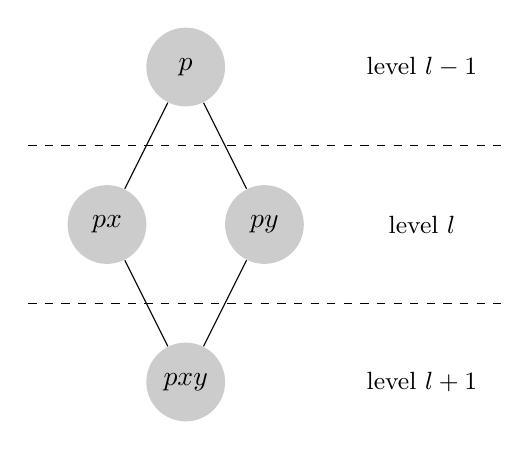
\begin{tikzpicture}
  [scale=1,auto=center,every node/.style={minimum size=1cm}]
    \node (p)  [circle,fill=black!20] at (4,10) {$p$};
    \node (n1) [circle,fill=black!20] at (3,8)  {$p x$};
    \node (n2) [circle,fill=black!20] at (5,8)  {$p y$};
    \node (n12)[circle,fill=black!20] at (4,6)  {$p x y$};


    \foreach \from/\to in {p/n1,p/n2,n1/n12,n2/n12}
      \draw (\from) -- (\to);

    \draw[dashed] (2,9) -- (8,9);
    \draw[dashed] (2,7) -- (8,7);

    \node (level0)[font=\small] at (7,10) {level $l-1$};
    \node (level1)[font=\small] at (7,8)  {level $l$};
    \node (level2)[font=\small] at (7,6)  {level $l+1$};
  \end{tikzpicture}
\end{center}



For every bucket $b_i$, there's a frequency $h_i$ in the histogram, we can calculate the conditional probability $p_i(x|p)$ and $p_i(y|p)$ assuming conditional independence given common parent $p$ in order to estimate $\hat{h_i}(p x y)$:

\begin{equation}
\begin{split}
 p_i(x|py) &= p_i(x|p) \\ 
 &= \cfrac{h_i(x)}{h_i(p)} \\ 
 p_i(y|px) &= p_i(y|p) \\ 
 &= \cfrac{h_i(y)}{h_i(p)} \\ \\ 
 \hat{h_i}(pxy) &= p_i(x|py)p_i(y|p)*h_i(p) \\ 
 &= p_i(x|p)h_i(y) \\ 
 \hat{h_i}(pxy) &= p_i(y|px)p_i(x|p)*h_i(p) \\ 
 &= p_i(y|p)h_i(x) 
\end{split}
\end{equation}

After that, we query the actual frequency distribution on the Knowledge Base and do an Pearson's chi-squared independence test. As null hypothesis and alternative hypothesis we have:

\begin{itemize}
 \item $H_0$ = \emph{$x$ and $y$ are conditionally independent given their common parent $p$}
 \item $H_1$ = \emph{$x$ and $y$ are conditionally dependent given their common parent $p$} 
\end{itemize}

  

Number of degrees of freedom is the number of buckets minus one:

\begin{center}
 $df=k-1$
\end{center}

We calculate the $\chi^2$ value:

\begin{equation}
 \chi^2=\sum_{i=1}^{k} \cfrac{(h_i - \hat{h_i})^2}{\hat{h_i}}
\end{equation}

\cite{Jaroszewicz02pruningredundant}

Then it's possible to obtain the p-value and check whether there's enough confidence to reject the null hypothesis $H_0$. In level 1 from \graphname, nodes can be directly pruned, on the other hand, for further levels, for a node to be pruned by independence, all the possible joins resulting the node must be independent. In level 2, for example, in order to prune the node $r a_1 b_1 c_1$, given that in level 1 the nodes $r a1 b1$, $r a1 c1$ and $r b1 c1$ were not pruned. All the three possible join combinations should fail the independence test, i.e.:

\begin{equation}
\begin{split} 
  freq(r a_1 b_1 c_1) &\approx freq(r a_1)p (r b_1|r a_1) p(r c_1|r a_1) \\ 
  &\approx  freq(r b_1) p(r a_1|r b_1) p(r c_1|r b_1) \\ 
  &\approx  freq(r c_1) p(r a_1|r c_1) p(r b_1|r c_1)  
\end{split}
\end{equation}

This applies to nodes at any level $l$, with $p \leq l$ parents and $C_{2}^{p}$ possible join pairs.

\section{Heuristics}

As seen in the previous sections, the number of nodes in \graphname grow exponentially with the number of categorical relations and its constants. For $n$ categorical relations, each with $m$ constants, the total number of nodes is $2^{n*m}$. Frequently, pruning by support and independence is not sufficient to make it feasible and it's necessary to apply heuristics to prune more aggressively.

As we are interested in categories that produces a subsets with a distribution different from the root and its super-categories (parent nodes, for the case of joining multiple categories), distribution divergence measures are a good option. Some of the state-of-the-art measures we can use are the following:

\begin{itemize}
 \item Kullback-Leibler \cite{Kullback51klDivergence}: 
    \begin{equation}
      D_{KL}(P||Q)=\sum_{\substack{i}}\ln\left(\cfrac{P(i)}{Q(i)}\right)*P(i)
    \end{equation}
 \item Chi-squared ($\chi^2$):
    \begin{equation}
      D_{\chi^2}(P||Q)=\sum_{\substack{i}}\cfrac{(P(i)-Q(i))^2}{P(i)}
    \end{equation}
 \item Jensen-Shannon \cite{17795}:
    \begin{equation}
      D_{JS}(P||Q)=\cfrac{1}{2}D_{KL}(P||M)+\cfrac{1}{2}D_{KL}(Q||M), 
    \end{equation}
\end{itemize}

Where $P$ and $Q$ are the distributions to be compared and $M=\cfrac{1}{2}(P+Q)$

As discussed in \cite{17795}, although Jensen-Shannon is computationally more expensivee, it has the advantage of being a symmetric and smoothed version of the Kullback-Leibler measure.

Nevertheless, using a divergence measure alone might also be problematic. Nodes with low support are very likely to present high divergence and when 






\section{Incorporating \graphname into Core ILP Algorithm}
